\documentclass[10pt]{article}

\usepackage[english]{babel}
\usepackage[utf8x]{inputenc}
\usepackage{amsmath}
\usepackage{amssymb}
\usepackage{amsfonts}
\usepackage{graphicx}
\usepackage[ruled,linesnumbered,noend]{algorithm2e}
\usepackage{empheq}
\usepackage{float}
\usepackage{enumitem}
\usepackage{tikz}
\usepackage[colorlinks=true,urlcolor=blue]{hyperref}

\title{Introduction to Machine Learning, Fall 2014 - Exercise session III}
\author{Rodion ``rodde'' Efremov, student ID 013593012}

\begin{document}
 \maketitle

\section*{Problem 1 (3 points)}
\color{blue}
Consider a binary classification task with two classes, `+` and `-`. The desired prediction is either one of the two classes,  or alternatively answering `don't know`, with the following cost matrix:
\color{black}
\begin{center}
\begin{tabular}{r|c|c|c|}
 & - & + & don't know \\
\hline
- & 0 & 10 & 2 \\
\hline
+ & 3 & 0 & 1 \\
\hline
\end{tabular}
\end{center}
\color{blue}
The goal is to minimize the expected cost (which is also the long-term arverage cost). You are given a classification method that returns a probabilistic prediction, i.e. for each new object the existing method gives you the probability $\alpha$ that the object belongs to class `+` (and hence $1 - \alpha$ is the probability that the object belongs to class `-`).

\noindent Give the optimal policy of answering `+`, `-`, or `don't know` for each object, as a function of the value of $\alpha$. That is, for any given value of $\alpha$ (for $0 \leq \alpha \leq 1$) what is the best answer of the three possibilities?
\color{black}

\subsection*{Solution}
So answering `+` has the cost of $0 \cdot \alpha + 10 (1 - \alpha) = 10 - 10\alpha$; the cost of ansering `-` is $3\alpha + (1 - \alpha) \cdot 0 = 3\alpha$; the cost of answering `don't know` is $1 \cdot \alpha + (1 - \alpha) \cdot 2 = 2 - \alpha$.

Next, let us compute all three intersection points between any pair of lines.
\begin{align*}
10 - 10\alpha &= 3\alpha \\
10 &= 13\alpha \\
\alpha &= \frac{10}{13}.
\end{align*}
The interesection $y$-coordinate is $\frac{30}{13} = 2\frac{4}{13}$, and thus, the point is $A = (\frac{10}{13}, 2\frac{4}{13})$.

\begin{align*}
10 - 10\alpha &= 2 - \alpha \\
8 &= 9 \alpha \\
\alpha &= \frac{8}{9}.
\end{align*}
The intersection $y$-coordinate is $2 - \frac{8}{9} = 1\frac{1}{9}$, and thus, the point is $B = (\frac{8}{9}, 1\frac{1}{9})$.

\begin{align*}
3\alpha &= 2 - \alpha \\
4\alpha &= 2 \\
\alpha &= \frac{1}{2}.
\end{align*}
The intesection $y$-coordinate is $3 \frac{1}{2} = \frac{3}{2}$, and thus, the point is $C = (\frac{1}{2}, \frac{3}{2})$.

After plotting $A$, $B$ and $C$, it becomes obvious that $A$ is above the line segment $BC$. Suppose that for any $I = A, B, C$, $I(x)$ is the $y$-coordinate of the point at position $x$ on line $I$, we are interested in the area below the function $\min (A(x), B(x), C(x))$. The function in question may be reconstructed from the three points we calculated:
\[
P(\alpha) = 
\begin{cases}
`-` & \text{if } \alpha \in [0, \frac{1}{2}] \\
`\text{don't know}` & \text{if } \alpha \in (\frac{1}{2}, \frac{8}{9}] \\
`+` & \text{if } \alpha \in (\frac{8}{9}, 1] \\
\end{cases}
\]
\section*{Problem 2 (3 points)}

\section*{Problem 3 (3 points)}

\section*{Problem 4 (9 points)}
\subsection*{(a)}
\color{blue}
Download the MNIST data from the course web page. In addition to the actual data, the package contains some functions for easily loading the data into Python/Matlab/Octave/R and for displaying digits. See the README files for details. Load the first $N=5,000$ images using the provided function.
\color{black}

\subsection*{Solution to (a)} 
Check!

\subsection*{(b)}
\color{blue}
Use the provided functions to plot a random sample of 100 handwritten digits, and show the associated labels. Verify that the labels match the digit images. (This is a sanity check that you have the data [is] in the right format.)
\color{black}

\subsection*{Solution to (b)}
\begin{center}
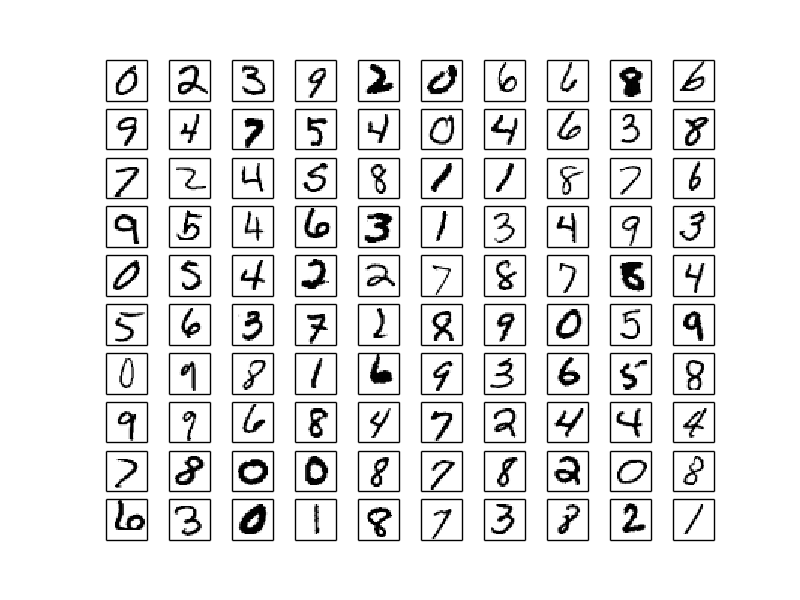
\includegraphics[scale=0.5]{100TestMnistImages}
\end{center}
The labels are:
\begin{center}
\begin{verbatim}
0 2 3 9 2 0 6 6 8 6 
9 4 7 5 4 0 4 6 3 8 
7 2 4 5 8 1 1 8 7 6 
9 5 4 6 3 1 3 4 9 3 
0 5 4 2 2 7 8 7 8 4 
5 6 3 7 2 8 9 0 5 9 
0 9 8 1 6 9 3 6 5 8 
9 9 6 8 4 7 2 4 4 4 
7 8 0 0 8 7 8 2 0 8 
6 3 0 1 8 7 3 8 2 1
\end{verbatim}
\end{center}

\subsection*{(c)}
\color{blue}
Divide the data into two parts: A `training set` consisting of the first 2,500 images (and associated labels), and a `test set` containing the remaining 2,500 images (and their associated labels).
\color{black}

\subsection*{Solution to (c)}
Check!

\subsection*{(d)}
\color{blue}
For each of the ten classes (digits 0-9), compute a class \textit{prototype} given by the mean of all the images in the training set that belong to this class. That is, select from the training set all images of class '0' and compute the mean image of these; this should look sort of like a zero. Do this for all ten classes, and plot the resulting images. Do they look like what you would expect?
\color{black}

\subsection*{Solution to (d)}
\begin{center}
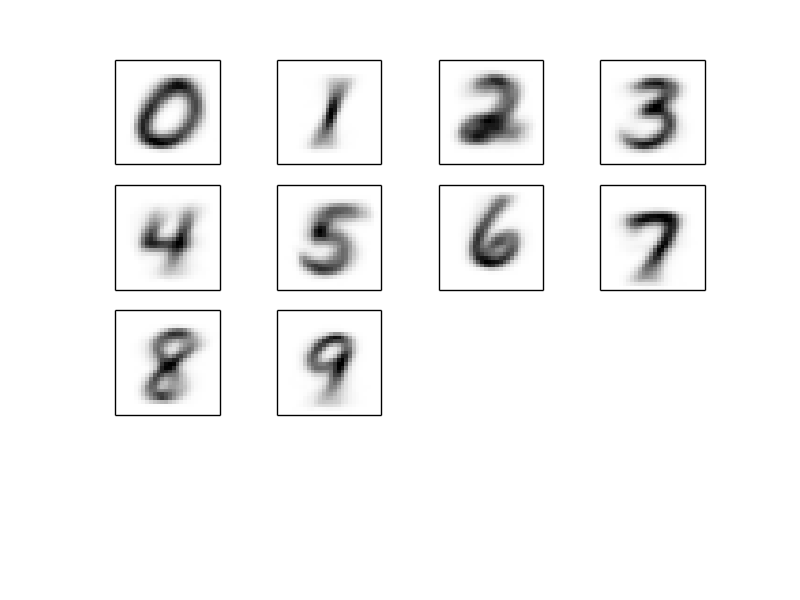
\includegraphics[scale=0.5]{MNISTPrototypes}
\end{center}
Obviously, the prototypes look good.

\subsection*{(e)}
\color{blue}
For each of the images in the test set, compute the Euclidean distance of the image to all 10 prototypes, and classify the test image into the class for which the distance to the prototype is the smallest.  So, if a test image is closer to the prototype for `3' than it is to the prototypes for any of the other digits, predict its class to be `3'.  Compute and display the resulting
\textit{confusion matrix}.
\color{black}

\subsection*{Solution to (e)}
The confusion matrix for the prototype-based classifier is
\begin{verbatim}
228   0   1   2   0   4   6   2   2   0
0   281   1   0   0   3   0   0   1   0
2    19 192   5   5   2   2   2  11   1
1     9   4 193   2  20   0   5  11   8
1     4   1   0 202   0   5   2   0  40
9    16   1  14  11 136   2   6   1  11
5    12  15   0   9   8 198   0   0   0
1    14   1   0  15   0   0 232   1  11
3    13   9  25   4  19   1   1 151  14
3     4   6   2  38   2   1  14   2 179
\end{verbatim}

\subsection*{(f)}
\color{blue}
Classify each of the test images with a nearest neighbor classifer: For each of the test images, compute its Euclidean distance to all (2,500) of the training images, and let the predicted class be the class of the closest training image. Compute and display the resulting confusion matrix.
\color{black}

\subsection*{Solution to (f)}
The confusion matrix of the kNN-classifier is
\begin{verbatim}
241   0   0   2   0   1   1   0   0   0
  0 283   0   0   1   1   0   1   0   0
  2   6 216   5   0   1   1   5   5   0
  0   0   3 221   2  11   2   4   5   5
  0   3   0   0 231   0   0   2   0  19
  5   3   0   6   0 183   5   1   1   3
  3   1   0   0   1   1 240   0   0   1
  0   3   2   0   6   0   0 257   0   7
  4   5   9  10   1   8   0   2 196   5
  2   2   0   2  12   1   2  11   0 219
\end{verbatim}

\subsection*{(g)}
\color{blue}
Compute and compare the error rates of both classifiers (the prototype-based classifier and the nearest neighbor classifier). Which is working better?  Based on the confusion matrix, which digits are confused with each other? Why do you think this is?
\color{black}

\subsection*{Solution to (g)}
The error rate of the prototype-based classifier is 0.2032 and the error rate of kNN is only 0.0852. Obviously, kNN surpasses prototype-based classifier. It seems that 4 and 9, 3 and 8 are problematic. Obviously, the aforementioned digits in each pair share a lot of common geometry.

\end{document}